\documentclass[tikz,border=2pt]{standalone}
\usepackage{amsmath,amssymb}
\usepackage{tikz}
\usetikzlibrary{arrows.meta}

\begin{document}
% For any two real numbers exactly one of x<y, x=y, x>y holds: on the line, x is to the left of y,
% on top of y, or to the right of y.
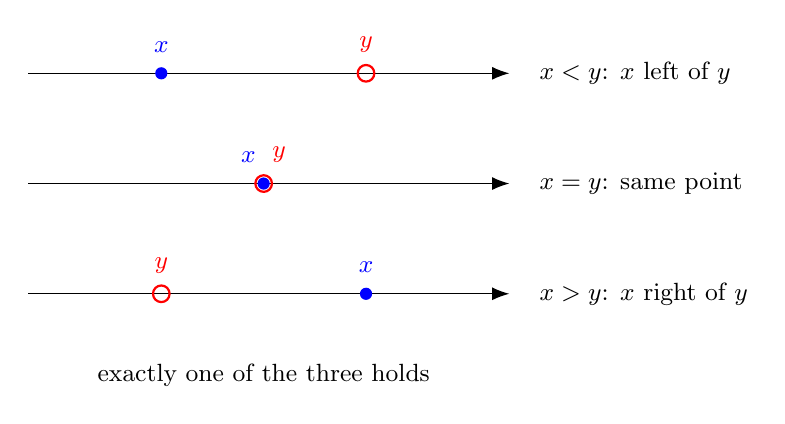
\begin{tikzpicture}[x=1.3cm, every node/.style={font=\small}]
	\foreach \y/\pa/\pb/\lab in {1.4/1/3/{$x<y$: $x$ left of $y$}, 0/2/2/{$x=y$: same point}, -1.4/3/1/{$x>y$: $x$ right of $y$}} {
		\draw[-{Latex[length=2.2mm]}] (-0.3,\y) -- (4.4,\y);
		\fill[blue] (\pa,\y) circle (2.2pt);
		\draw[red, thick] (\pb,\y) circle (3pt);
		\node[anchor=west] at (4.6,\y) {\lab};
	}
	\node[blue, above=4pt] at (1,1.4) {$x$}; \node[red, above=4pt] at (3,1.4) {$y$};
	\node[blue, above=4pt] at (1.85,0) {$x$}; \node[red, above=4pt] at (2.15,0) {$y$};
	\node[red, above=4pt] at (1,-1.4) {$y$}; \node[blue, above=4pt] at (3,-1.4) {$x$};
	\node[below=22pt, align=center] at (2,-1.4) {exactly one of the three holds};
\end{tikzpicture}
\end{document}
